\emph{Links2} è un browser testuale da terminale. Permette di visualizzare il sito solo con una struttura molto minimale. \\
Per garantire una buona navigazione generale, da parte di tutti, deve essere possibile utilizzare il sito anche tramite un browser testuale.\\
Quindi, se è possibile navigare facilmente con links2 allora la probabilità che una persona con disabilità visive abbia difficoltà a navigare
all'interno del sito scende di molto. Infatti tramite links2 sappiamo determinare anche il comportamento di uno screen reader.\\
Questo tool inoltre ci ha permesso di capire il comportamento del sito in mancanza di immagini.\\

\begin{figure}[!h]
	\centering
	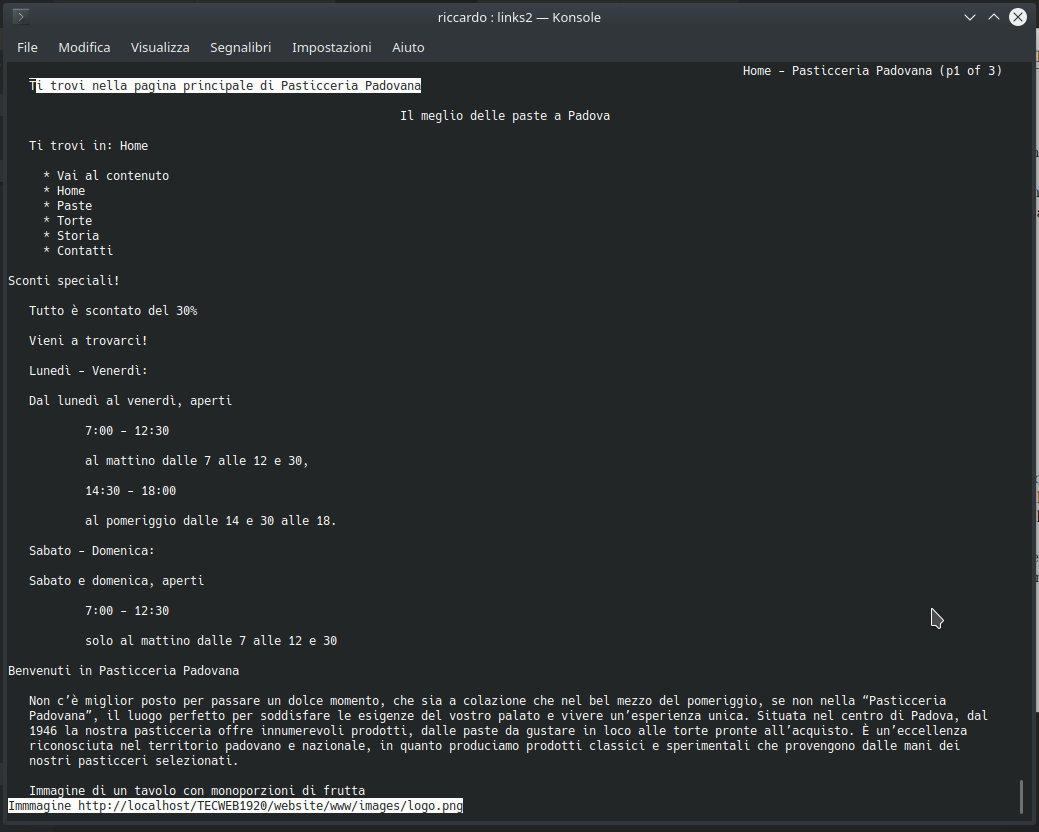
\includegraphics[width=0.7\linewidth]{sezioni/FaseTest/Immagini/links2.png}\\
	\caption{links2 – terminal browser}
	\label{Fig:links2}
\end{figure} 
\newpage